%%%%%%%%%%%%%%%%%%%%%%%%%%%%%%%%%%%%%%%%%%%%%%%%%%%%%%%%%%%%%%%%%%%%%%%%%%%%%%%%%%%%%%%%
%
%  TeX template file for Transactions of JSASS,
%                        Aerospace Technology Japan,
%                        ISTS Special Issue
%                        APISAT Special Issue
%
%                 Ver.2.0  May 2016, JSASS Publication Committee
%%%%%%%%%%%%%%%%%%%%%%%%%%%%%%%%%%%%%%%%%%%%%%%%%%%%%%%%%%%%%%%%%%%%%%%%%%%%%%%%%%%%%%%%
%\documentclass[TJSASS]{tjsass} % draft for Transactions of JSASS
%\documentclass[ATJ   ]{tjsass} % draft for Aero. Tech. Japan
\documentclass[ISTS  ]{tjsass} % draft for ISTS
%\documentclass[APISAT]{tjsass} % draft for APISAT

%\documentclass[TJSASS, pubform]{tjsass} % publication paper for Transactions of JSASS
%\documentclass[ATJ   , pubform]{tjsass} % publication paper for Aero. Tech. Japan
%\documentclass[ISTS  , pubform]{tjsass} % publication paper for ISTS
%\documentclass[APISAT, pubform]{tjsass} % publication paper for APISAT

%%%%%%%%%%%%%%%%%%%%%%%%%%%%%%
%---Required Packages---
%%%%%%%%%%%%%%%%%%%%%%%%%%%%%%
%The packages below should be installed on your PC
\usepackage{graphicx}
\RequirePackage{multicol}
\RequirePackage{amsmath}
\RequirePackage[varg]{txfonts}
\RequirePackage{bm}
\RequirePackage{array}
%\RequirePackage{color}
\RequirePackage{tjsasscite}
\usepackage[hang]{footmisc}
\newcommand{\bhline}[1]{\noalign{\hrule height #1}}
\usepackage[a4paper,total={176mm,247mm},top = 30mm,left=17mm]{geometry}
\usepackage{tabularx}
\usepackage{multirow}

%%%%%%%%%%%%%%%%%%%%%%%%%%%%%%
%---Publication Info.---
%%%%%%%%%%%%%%%%%%%%%%%%%%%%%%
\pubyear{2017}% year of publication
\bookvolume{14}% volume
\bookissue{ists31}% issue
\session{d} % session category if ists paper
\setcounter{page}{1}% starting page number
\titleheadertrue% title for header
\receiveddate{April 17th, 2017}%
%\revisiondate{August 10th, 2017}
%\accepteddate{September, 20th, 2017}
\confinfo{presented at 26th ISSFD, June 8th, 2017}
%\AEname{J. Aero} %Associate Editor name
\pagenumbering{arabic}
\setcounter{page}{1}
\pagestyle{plain}
%%%%%%%%%%%%%%%%%%%%%%%%%%%%%%
%---Set up Title & Author---
%%%%%%%%%%%%%%%%%%%%%%%%%%%%%%

\title{Benchmarking the Collocation Stand-Alone Library and Toolkit (CSALT)}% paper title
\subtitle{}% paper subtitle only when necessary
%
%%%%%% put author's name in \author{} following the rules below.
%%  \NAME{first name}{last name}   %last name is converted to capital letters.
%%  \thanksNum{affiliation}
%
\author{\NAME{Steven}{Hughes},\thanksNum{1)}\CorresAuthor{steven.p.hughes@nasa.gov}
\NAME{Jeremy}{Knittel},\thanksNum{1)}
\NAME{Wendy}{Shoan},\thanksNum{1)}
\NAME{Youngkwang}{Kim},\thanksNum{2)}
\NAME{Claire}{Conway},\thanksNum{3)} and
\NAME{Darrel}{Conway}\thanksNum{3)}
}% author&affiliation
%
%%%%%% \thanksOrg{}
%%%%%%   affiliations are automatically numbered.
%
\thanksOrg{NASA Goddard Space Flight Center, USA}% affiliation 1
\thanksOrg{Yonsei University, South Korea}% affiliation 2
\thanksOrg{Thinking Systems Inc., USA}
%
%%%%%%%%%%%%%%%%%%%%%%%%%%%%%%
%---Abstract and Keywords---
%%%%%%%%%%%%%%%%%%%%%%%%%%%%%%
%
\begin{abstract}
This paper describes the processes and results of Verification and Validation (V\&V) efforts for the Collocation Stand Alone Library and Toolkit (CSALT).  We describe the test program and environments, the tools used for independent test data, and comparison results. The V\&V effort employs classical problems with known analytic solutions, solutions from other available software tools, and comparisons to benchmarking data available in the public literature.  Presenting all test results are beyond the scope of a single paper.  Here we present high-level test results for a broad range of problems, and detailed comparisons for selected problems.
\end{abstract}
%
\keywords{optimal control, trajectory optimization, collocation}
%
%%%%%%%%%%%%%%%%%%%%%%%%%%%%%%
%---Main Document Start---
%%%%%%%%%%%%%%%%%%%%%%%%%%%%%%
%
\begin{document}
\maketitle

\section*{Nomenclature}

\vbox{\noindent\setlength{\tabcolsep}{0mm}%
\begin{tabular}{p{25mm}cl} %
\hfil$\mathbf{z}$\hfil & :\hspace{4mm} & decision vector \\
\hfil$\mathbf{f}$\hfil & :\hspace{4mm} & NLP functions \\
\hfil$\mathbf{q}$\hfil & :\hspace{4mm} & optimal control functions \\
\hfil$\mathbf{x}$\hfil & :\hspace{4mm} & state vector \\
\hfil$\mathbf{u}$\hfil & :\hspace{4mm} & control functions \\
\hfil$J$\hfil & :\hspace{4mm} & cost function \\
\hfil$t$\hfil & :\hspace{4mm} & time \\
% \frac{\partial\mathbf{f}}{\partial} = \mathbf{A} + \mathbf{B} \frac{\partial\mathbf{q}}{\partial\mathbf{x}}
\end{tabular}}

% \noindent{Subscripts}
%
% \vbox{\noindent\setlength{\tabcolsep}{0mm}%
% \begin{tabular}{p{25mm}cl}
% \hfil$0$\hfil & :\hspace{4mm} & initial \\
% \hfil$\mathrm{f}$\hfil & :\hspace{4mm} & final
% \end{tabular}}

\section{Introduction}
The Collocation Stand Alone Library and Toolkit (CSALT) is a C++ library that employs collocation for solving the optimal control problem\cite{Betts:a}. The library contains approximately 17,000 Source Lines of Code (SLOC) for the CSALT library and about 17,000 SLOC reused from utilities in the General Mission Analysis Tool (GMAT)\cite{Hughes:a}.  The system has (loose) dependencies on the Boost C++ library for sparse matrix arithmetic, and SNOPT\cite{Gill:a} for nonlinear programming.  The software was developed in collaboration between GSFC engineers and software developers, GSFC support contractors, and the Korea Aerospace Research Institute (KARI) and is licensed using the Apache License 2.0.

CSALT is under active development.  It currently supports 6 transcriptions ranging from trapezoid\cite{Betts:a} to Radau orthogonal collocation\cite{Rao:a} employing a ph mesh refinement algorithm\cite{Rao:c}.  The user interface is object-oriented, and is similar to, and inspired by, the user interface in PSOPT\cite{Becerra:a}.

This paper documents the benchmarking and testing performed on CSALT to date, focusing on system accuracy and robustness for multi-phase optimal control problems (performance benchmarking, while important, will be addressed in future work).  Our benchmarking efforts heavily reference standard problems in the literature.  We refer the reader to those references for problem specific details and, except in a few limited cases, we do not repeat well known problem specifications in this paper. Our benchmarking effort employs several external truth sources including comparison to exact analytic solutions when available, comparison to solutions from GPOPS II\cite{Rao:a}, SOS\cite{Betts:c}, and PSOPT\cite{Becerra:a}, and, for low thrust space trajectory optimizations, comparison to industry standard benchmarking problems documented by Horsewood and Dankanich.\cite{Horsewood:a}

Current and near term efforts on CSALT are focused on integration into NASA’s General Mission Analysis Tool (GMAT) and will address  performance benchmarking and improvements, and implementation of additional functionality in the core CSALT library.

\section{Optimal Control Problems}

Optimal control problems have been studied extensively over the past half-century with applications in all areas of engineering. Fundamentally, an optimal control problem is any that can be expressed as a system of ordinary differential equations, governed by either discrete or continuously varying control inputs.

If an optimal control problem is sufficiently complex, and cannot be solved analytically, numerical methods must be applied. There are two main classes of numerical methods: indirect and direct. For an overview of trajectory optimization methods we refer the reader to Refs. \citeN{Stryk:a} and \citeN{Betts:a}.

For any optimal control problem, the general mathematical strategy is to minimize a cost function, $J$ (written in what is called the Bolza form \cite{Betts:a}:
%
\begin{equation}
   J =\Phi\left(\mathbf{x}(t_o),t_o,\mathbf{x}(t_f),t_f) \right) +  \int_{t_o}^{t_f} \lambda(x(t),u(t),t) dt
\end{equation}
%
subject to the ordinary differential equations describing the system,
%
\begin{equation}
   \dot{\mathbf{x}}(t) = \mathbf{a}(\mathbf{x}(t),\mathbf{u}(t),t)
\end{equation}
%
algebraic path constraints,
%
\begin{equation}
   \mathbf{p}(\mathbf{x}(t),\mathbf{u}(t),t) \leq \mathbf{0}
\end{equation}
%
%
and boundary conditions,
%
\begin{equation}
   \mathbf{b}(\mathbf{x}(t_o),\mathbf{u}(t_o),\mathbf{x}(t_f),\mathbf{u}(t_f),t_o,t_f) \leq   \mathbf{0}
\end{equation}
%
where $\mathbf{x}$ is the state vector, and $\mathbf{u}$ is the vector of controls.

\section{Current CSALT Capability}

CSALT employs collocation to solve the optimal control problem.  Collocation converts an optimal control problem to a large, sparse Non-Linear Programming (NLP)\cite{Nodecal:a} problem.  The differential equations in the optimal control problem are converted to a set of differential algebraic equations whose solution approximates the solution to the differential equations.   The approximation accuracy is governed by the transcription (how the differential equations are expressed as a system of algebraic equations) and how accurately those equations are solved.  CSALT employs both low and high order transcriptions that are all implicit integration schemes.  The transcriptions currently supported are Trapezoid, Hermite Simpson, Lobatto IIIa\cite{Betts:e} methods of order 4, 6, and 8, and Radau orthogonal collocation.   CSALT casts all transcriptions in the form proposed by Betts (see Ref. \citeN{Betts:a}, pg. 146):
%
\begin{equation}
\mathbf{f} = \mathbf{A} \mathbf{z} + \mathbf{B} \mathbf{q} \label{Eq:BettsNLPForm}
\end{equation}
%
where $\mathbf{A}$ and $\mathbf{B}$ are constant matrices dependent upon the transcription, $\mathbf{z}$ is the decision vector, $\mathbf{f}$ is the vector of nonlinear programming functions, and $\mathbf{q}$ is the vector of optimal control functions evaluated at the discretization points.   The system currently supports Mayer, Lagrange, or Bolza form cost functions, algebraic path constraints, and algebraic point constraints.  Optimization parameters include state, control, and time parameters.  Integral constraints, static, and integral variables will be implemented within the next year.

\subsection{Derivatives and Sparsity Determination}

Sparse derivatives are supplied to the NLP solver by differentiating Eq.~(\ref{Eq:BettsNLPForm}) resulting in
%
\begin{equation}
\frac{\partial\mathbf{f}}{\partial\mathbf{z}} = \mathbf{A} + \mathbf{B} \frac{\partial\mathbf{q}}{\partial\mathbf{z}}   \label{Eq:BettsJacobianForm}
\end{equation}
%
The derivatives are computed using sparse matrix representations of the arrays, where the optimal control problem derivatives $\frac{\partial\mathbf{q}}{\partial\mathbf{z}}$ can optionally be provided by the user.  If some or all of the optimal control derivatives are not provided, CSALT performs finite differencing of the optimal control functions.

NLP sparsity is determined using
%
\begin{equation}
    \text{Sparsity}(\frac{\partial\mathbf{f}}{\partial\mathbf{z}}) = \text{Sparsity}(\mathbf{A} + \mathbf{B} \frac{\partial\mathbf{q}}{\partial\mathbf{z}})   \label{Eq:BettsSparsityForm}
\end{equation}
%
where the sparsity of the users optimal control functions are determined by randomly varying the decision variables within the user-defined bounds on those variables.

\subsection{Scaling}

The NLP problem can be solved with greater efficiency if it is scaled properly. If the magnitudes of the decision vector and NLP functions are not consistent, then so too will be the magnitudes of the derivatives. This will then unnaturally weight the optimization algorithm steps. Further, if a given constraint is poorly scaled relative to other constraints, then it will be difficult to reach feasibility. These challenges can be improved with proper problem scaling. The scaling in CSALT follows the method proposed by Betts (\citeN{Betts:b} ( pg. 45). First, the decision vector values are all transformed using their bounds to the interval [-1/2,1/2]. Second, all defect constraints are scaled using a matching transformation. Finally, all other constraint functions are scaled such that the norm of the associated row of constraint function derivatives in the Jacobian is unity. Note that the scaling factors are determined based on the magnitudes of the Jacobian of the initial guess, further increasing its importance.

\subsection{Mesh Refinement}

Currently, CSALT supports mesh-refinement for the Radau orthogonal collocation method. For the Radau orthogonal collocation method, a mesh refinement algorithm presented in Ref. \citeN{Rao:c} is implemented in CSALT. The role of the mesh-refinement algorithm is to apply proper changes to the discretization (i.e., the length of the mesh interval and the degree of the approximating polynomial) in order to satisfy the user-defined tolerance on the relative collocation error. The relative collocation error represents the quality of the collocated solution, and the mesh refinement algorithm estimates the relative collocation error as the difference between the approximating polynomials and the quadrature integration results of the dynamics functions. According to Rao\cite{Rao:c}, the required polynomial degree of a mesh interval is obtained as follows:
%
\begin{equation}
   P^k= \log_{N^k}\left( \frac{e}{\epsilon}\right), \hspace{0.1 in}  k=0,1,2,...,k_{max}
\end{equation}
%
where ${N^k}$ is the current polynomial degree after the $k$-th mesh refinement, $P^k$ is the required polynomial degree change, $\epsilon$ is the collocation error tolerance, $k_{max}$ is the maximum number of mesh refinement iterations, and $e$ is the current estimate of relative collocation error. In addition, there are static tuning parameters  $N_{min}$ and $N_{max}$ of the mesh refinement algorithm that define the boundaries of the polynomial degree such that:
%
\begin{equation}
   N_{min} \leq N \leq N_{max}, \hspace{0.1 in}  \mbox{for any $k$}
\end{equation}
%
CSALT adopts $N_{min}$=3, and $N_{max}$=14 based on the empirical data provided in Ref. \citeN{Rao:c}. If $N^k+P^k \leq N_{max}$, the degree of the polynomial is updated as using
%
\begin{equation}
   N^{k+1} = N^k+P^k
\end{equation}
%
If $N^k+P^k > N_{max}$, the mesh refinement algorithm divides the mesh interval into subintervals having $N^{k+1}=N_{min}$. The number of subintervals $B$ is given as follows:
%
\begin{equation}
   B=max(\left[\frac{N^k+P^k}{N_{min}}\right],2)
\end{equation}

\section{Benchmarking Results}

Comparing solutions to optimal control problems is complicated by the fact that there are several possible sources of error that can account for differences in solutions between different approaches and tools and because there are subjective and conflicting measures of performance, like accuracy and run-time evaluations.   Perhaps the most obvious issue is implementation error, which any benchmarking effort should catch.   Other sources of error include errors in the approximation employed, errors in the solution of the approximate equations, and, when using discretized solutions, errors caused by interpolation to common discretization points generated by different approaches or tools.

The benchmarking approach we employ is designed to ensure the errors above can be characterized, and, most importantly, numerical or approximation errors are not masking problems in implementation.  We have selected 17 benchmarking problems from the literature.  For all problems, we provide a comparison of optimal cost provided by CSALT to the optimal cost provided by an independent, trustworthy source.  Second, we include detailed comparisons for several problems that have known, exact solutions and show the maximum errors in state and control parameters between CSALT and the analytic solution. Comparison against exact solutions avoids the need to interpret differences between approximate solutions or interpolation to common times because the analytic solution allows double precision evaluation of the state and control at the same times used by the CSALT library.   We also show comparisons between CSALT and other collocation tools and show agreement to within expected accuracy, given tolerances used in the NLP problem and interpolation of the solutions.  Finally, we show applications to interplanetary low thrust benchmarks solved using the Calculus of Variations and other numerical methods.

In the next section, we identify specifications of the benchmarking problems.

\subsection{Problem Specification Sources}

For the purposes of benchmarking we have selected 15 test problems solved either exactly or with other collocation software systems with solutions documented in the open literature.  The list of problems is shown in Table \ref{table:high_level_comparison}, along with the optimal cost from CSALT and the truth source.   The problem specifications are openly available in Refs. \citeN{Betts:d}, \citeN{Becerra:a}, \citeN{Garg:a}, and \citeN{Hull:a} and we refer the reader to those specifications for details.  The page numbers in Table \ref{table:high_level_comparison} point to the pages in the preceding references that contain the configuration used for benchmarking, as in some cases, multiple configurations or parameterizations can be employed to solve a given problem.

The problems selected contain multiple phase problems, problems with Single Input Single Output (SISO) and Multiple Input Multiple Output (MIMO) control configurations, and singular optimal control problems.  There are problems with state and control path constraints and end point constraints and problems with algebraic and integral cost.  Some problems deserve special explanation.  In particular, the form of the Goddard Rocket problem solved here is a three phase singular arc problem that incorporates optimality conditions derived from the Calculus of Variations.  Additionally, there are two problems with exact analytic solutions. Rigorous comparisons for those problems are investigated in the next section.

The results in Table \ref{table:high_level_comparison} and  \ref{table:high_level_comparison2} show excellent agreement with independent solutions.  The tables contain the optimal cost value from CSALT and the independent truth source.   In general, CSALT agrees with the truth sources to the level of precision provided in the output of those systems.  Notably, the comparison with analytic solutions shows agreement on the order of 1E-12 relative error.
%
\begin{table}
	\centering
	\caption{High level optimal control comparisons}
	\label{table:high_level_comparison}
	\begin{tabularx}{\columnwidth}{lXXX}\bhline{.8pt}
                         \textbf{Test Case}  & Rayleigh    & Rayleigh                              & Goddard                 \\
                                             & (Control    & (Control)                             & Rocket                  \\
                                             & Constraint) & (+ State                              &                         \\
                                             &             & Constraint)                           &                         \\\hline
        \multirow{2}{*}{\textbf{Reference}} & SOS                          & SOS                                   & SOS/GPOPS               \\
                            & (pg. 237)                    & (pg. 241)                             & (pg. 122)               \\
        \textbf{CSALT}      & 44.7209344                   & 44.80444625                           & 18550.8718              \\
        \textbf{``Truth''}  & 44.7209362                   & 44.80444330                           & 18550.8710              \\
        \textbf{Difference} & -4.03E-08                    & 6.59E-08                              & -8.57E-09               \\\bhline{.8pt}
        \textbf{Test Case}  & Hyper-                       & Conway                                & Lin. Tangent            \\
                            & sensitive                    & Orbit                                 & Steering                \\\hline
        \multirow{2}{*}{\textbf{Reference}} & SOS/GPOPS                    & SOS                                   & SOS/GPOPS               \\
                            & (pg. 47)                     & (pg. 181)                             & (pg. 166)               \\
        \textbf{CSALT}      & 6.72411391                   & 0.0951233814                          & 0.55457088              \\
        \textbf{``Truth''}  & 6.72412325                   & 0.0951233834                          & 0.55457088              \\
        \textbf{Difference} & -1.39E-06                    & -2.11E-08                             & -1.19E-09               \\\bhline{.8pt}
        \textbf{Test Case}  & Brachisti                    & Bryson                                & Schwartz                \\
                            & -chrone                      & Denham                                &                         \\\hline
        \multirow{2}{*}{\textbf{Reference}} & SOS/GPOPS                    & GPOPS/PSOPT                           & PSOPT                   \\
                            & (pg. 53)                     & (pg. 126)                             & (pg. 373)               \\
        \textbf{CSALT}      & 0.31248013                   & 3.999991270                           & 2.49E-14                \\
        \textbf{``Truth''}  & 0.31248013                   & 3.999994899                           & 4.63E-15                \\
        \textbf{Difference} & 2.37E-09                     & -9.07E-07                             & 4.38E+00                \\\bhline{.8pt}
        \textbf{Test Case}  & Interior Point               & Bryson Max Range                      & Obstacle Avoidance      \\\hline
        \multirow{2}{*}{\textbf{Reference}} & PSOPT                        & PSOPT                                 & PSOPT                   \\
                            & (pg. 202)                    & (pg. 132)                             & (pg. 306)               \\
        \textbf{CSALT}      & 0.92053144                   & -1.7123149                            & 4.571044                \\
        \textbf{``Truth''}  & 0.92053140                   & -1.7123160                            & 4.571044                \\
        \textbf{Difference} & 4.53E-08                     & -6.57E-07                             & 0.00E+00                \\\bhline{.8pt}
        \textbf{Test Case}  & Moon                         & Rau                                   & Hull                    \\
                            & Lander                       & Automatica                            & Problem 9.5             \\\hline
        \multirow{2}{*}{\textbf{Reference}} & PSOPT                        & Analytic                              & Analytic                \\
                            & (pg. 306)                    &                                       &                         \\
        \textbf{CSALT}      & 1.42031885                   & -8.96380E-3                           & -8.33333E-2              \\
        \textbf{``Truth''}  & 1.42037700                   & -8.96380E-3                           & -8.33333E-2                     \\
        \textbf{Difference} & -4.09E-05                    & 4.70E-12                              & 4.00047-12                   \\\bhline{.8pt}
	\end{tabularx}
\end{table}
%
\begin{table}
	\centering
	\caption{High level optimal control comparisons}
	\label{table:high_level_comparison2}	\begin{tabularx}{\columnwidth}{Xcc}\bhline{.8pt}
        \textbf{Test Case}                    & \textbf{``Truth'' Source} & \textbf{Difference}\\\hline
        Rayleigh \\ (Control Contraint)          & SOS                       & -4.03E-08\\
        Rayleigh \\ (Control + State Constraint) & SOS                       & 6.59E-08\\
        Goddard Rocket                        & SOS /GPOPS                & -8.57E-09\\
        Hypersensitive                        & SOS /GPOPS                & -1.39E-06\\
        Conway Orbit                          & SOS                       & -2.11E-08\\
        Linear Tangent Steering               & SOS /GPOPS                & -1.19E-09\\
        Brachistichrone                       & SOS /GPOPS                & 2.37E-09\\
        Bryson Denham                         & GPOPS /PSOPT              & -9.07E-07\\
        Schwartz                              & PSOPT                     & 4.38E+00\\
        Interior Point                        & PSOPT                     & 4.53E-08\\
        Bryson Max Range                      & PSOPT                     & -6.57E-07\\
        Obstacle Avoidance                    & PSOPT                     & 0.00E+00\\
        Moon Lander                           & PSOPT                     & -4.09E-05\\
        Rau Automatica                        & Analytic                  & 4.70E-12\\
        Hull Problem 9.5                      & Analytic                  & 4.00E-12\\\bhline{.8pt}
	\end{tabularx}
\end{table}

\subsection{Comparison to Exact Solutions}

For high precision comparisons we selected two optimal control problems with known analytic solutions; an example problem presented by Hull \cite{Hull:a} (problem 9.5), and a problem presented by Garg and Rao \cite{Garg:a}. The analytic solutions for state and control are presented in those references.  Figure \ref{fig:rauCompare} shows a plot of the CSALT solution and the exact solution for the Rau Automatica problem and both are qualitatively similar.   Table \ref{table:exact_solutions} shows the maximum relative state and control errors for both test problems.  In both cases, state and control agree to at least 1e-6 and often much better.  These solutions were generated with tolerances for optimality, and feasibility in SNOPT of 1e-8, and mesh refinement tolerances of 1e-6.   Even better agreement is achieved when tolerances are tightened, but at a significant increase in run time.
%
\begin{table}
    \centering
    \caption{CSALT Comparison to Exact Solutions}\label{table:exact_solutions}
    \begin{tabular}{lcc}\bhline{.8pt}
        Problem & Max. State Error & Max. Control Error \\\hline
        Hull Problem 9.5 & 2.876e-09 & 2.817e-08 \\
        Rao Automatica & 5.109e-08 & 2.391e-06\\\bhline{.8pt}
    \end{tabular}
\end{table}
%
\begin{figure} [t!]
    \centering
    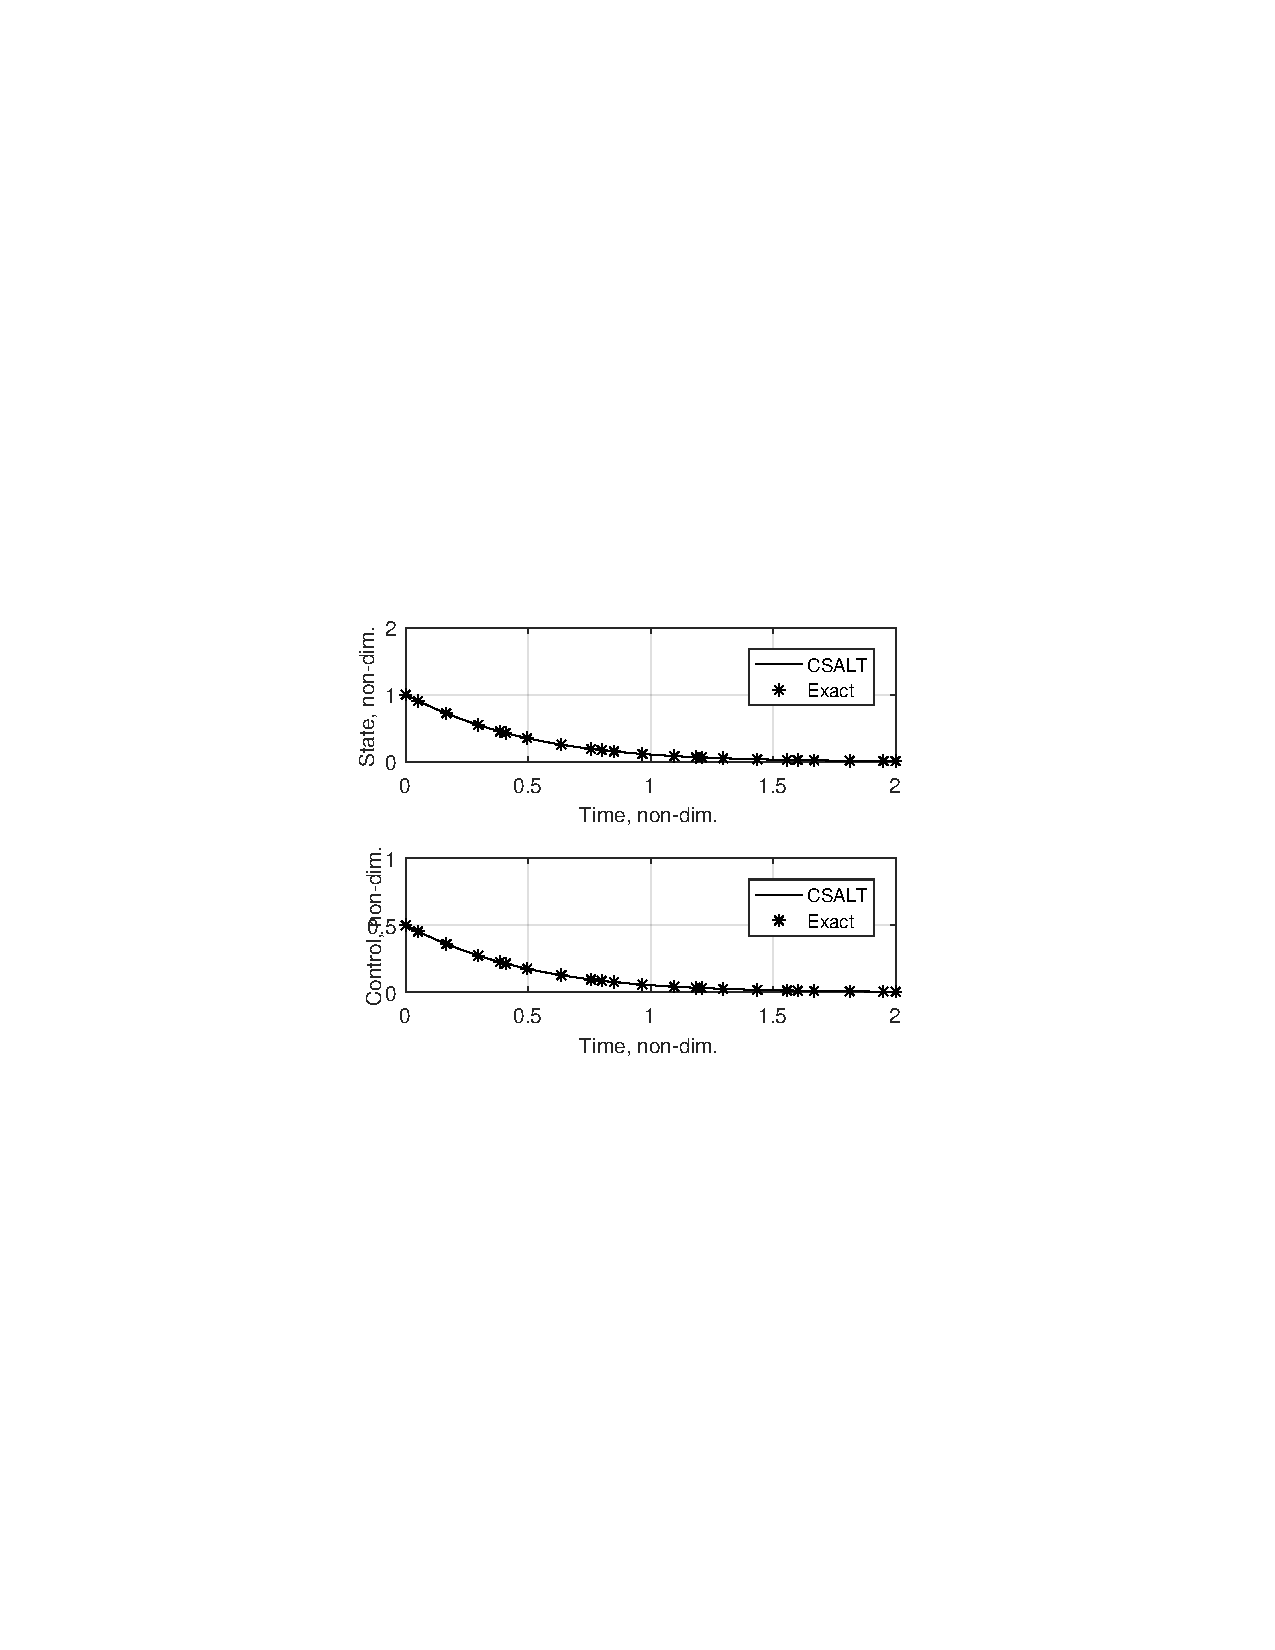
\includegraphics[width=\columnwidth]{../Figures/Rau_Compare}
    \caption{State and Control Comparison for Rao Automatica}
    \label{fig:rauCompare}
\end{figure}

\subsection{Comparison to Other Collocation Tools}

We selected three problems for detailed comparisons.   The Conway orbit raising problem is a classical problem well known in the literature, the Goddard Rocket problem is a stressing case because it contains a singular arc, and the Hypersensitive problem, because it is a stressing case for mesh refinement.   For each problem we present qualitative graphical comparisons and quantitative comparisons by showing the maximum state and control differences between CSALT and the solution generated by either SOS or GPOPSII.  Note, comparison of the cost solution was discussed in the problem overview section.

Figures \ref{fig:hyper_state} and  \ref{fig:hyper_control} show relevant portions of the state and control history for the Hypersensitive orbit problem computed by CSALT and GPOPSII.  For the hypersensitive problem, the dynamics change rapidly at the beginning and end of the time window, and are nearly constant for the middle portions of the window and the solutions between CSALT and GPOPSII are similar. Table \ref{table:coll_solutions} shows the maximum relative state and control difference of 4.305e-02 and 2.911e-01 respectively. These are larger than desirable.  We believe the difference is due to interpolation to common discretization times and this is supported by comparing the agreement between SOS and GPOPS-II solutions where the maximum relative state and control differences are 3.54e-01 and 1.037 respectively when interpolated to common discretization times using cubic splines.
%
\begin{figure}[h]
    \centering
    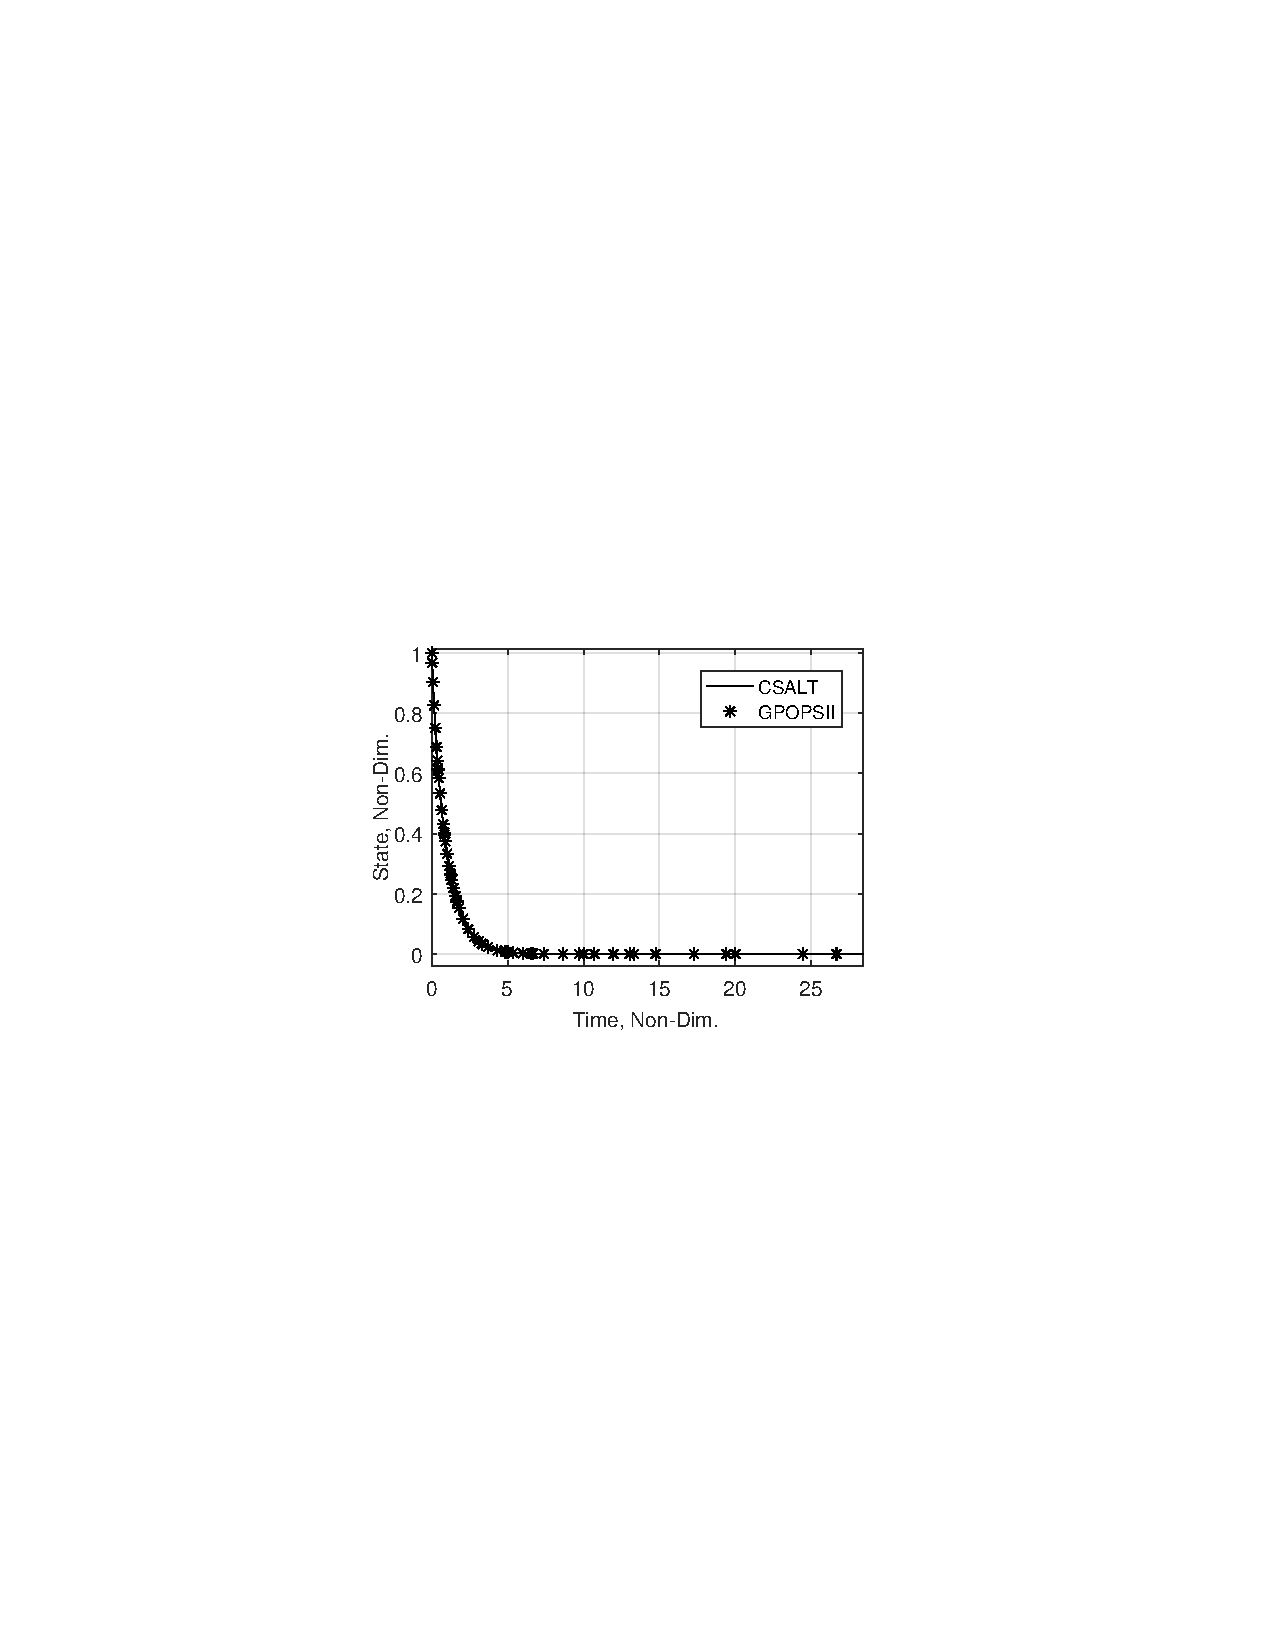
\includegraphics[width=\columnwidth]{../Figures/HyperSensitive_StateCompare}
    %\special{psfile= ../Figures/HyperSensitive_StateCompare.eps hoffset= 0 voffset=-150 hscale=90 vscale=90}
    \caption{State Comparison for Hypersensitive Problem}
    \label{fig:hyper_state}
\end{figure}
%
\begin{figure}[h]
    \centering
    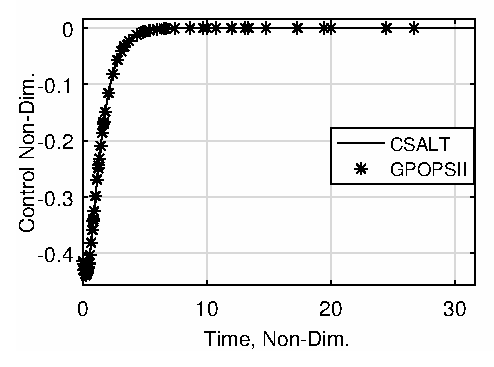
\includegraphics[width=\columnwidth]{../Figures/HyperSensitive_ControlCompare}
    \caption{Control Comparison for Hypersensitive Problem}
    \label{fig:hyper_control}
\end{figure}
%
\begin{table}
    \centering
    \caption{CSALT Comparison to Other Collocation Tools}\label{table:coll_solutions}
    \begin{tabular}{lccc}\bhline{.8pt}
        Problem Name & Tool & Max. Rel.  & Max. Rel.  \\
                     &      &  State Error &  Control Error \\\hline
        Goddard  & SOS  & 6.863e-07 & 2.191e-08 \\
        Hypers. & GPOPSII & 4.305e-02 & 2.911e-01\\
        Conway & SOS& 9.814e-06 & 1.610e-02\\\bhline{.8pt}
    \end{tabular}
\end{table}

Figures \ref{fig:conway_state} and \ref{fig:conway_control} show the state and control history for the Conway orbit problem computed by CSALT and SOS.  The problem is a finite thrust orbit raising problem, and the solution results in three orbital revolutions.  The solutions are qualitatively similar and differences cannot be seen on the scale of the graphics. Table \ref{table:coll_solutions} contains data illustrating the maximum state and control differences between the two systems. The state agreement is excellent with a maximum relative difference of 9.814e-06, while the maximum relative control difference is 1.610e-02.
%
\begin{figure}[h]
    \centering
    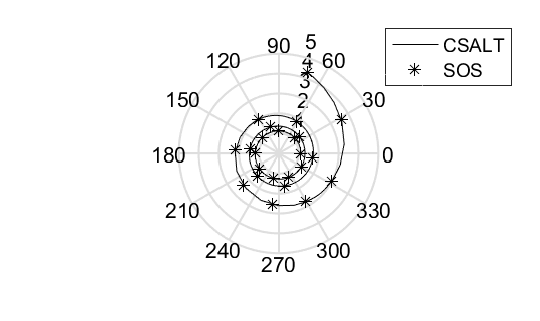
\includegraphics[width=\columnwidth]{../Figures/ConwayOrbit_StateCompare.eps}
    \caption{State Comparison for Conway Orbit Problem}
    \label{fig:conway_state}
\end{figure}
%
\begin{figure}
    \centering
    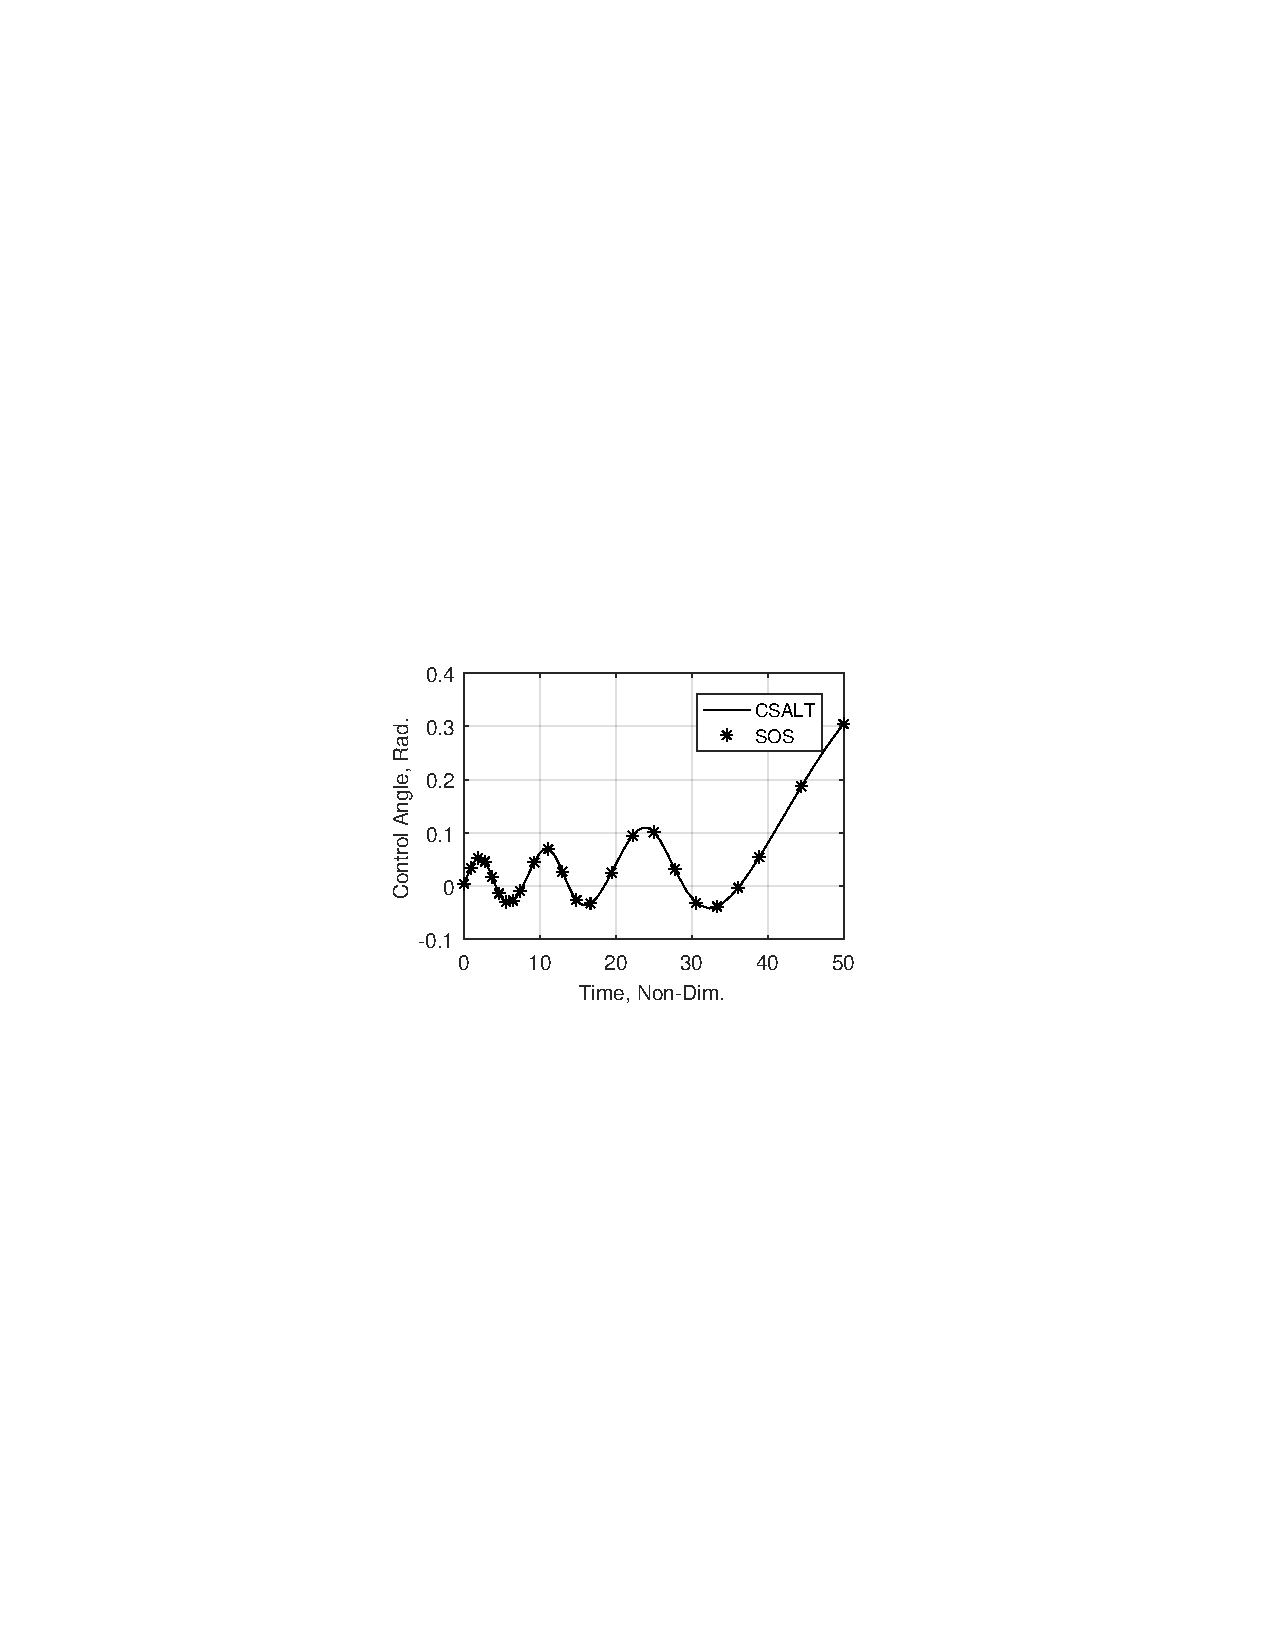
\includegraphics[width=\columnwidth]{../Figures/ConwayOrbit_ControlCompare}
    \caption{Control Comparison for Conway Orbit Problem}
    \label{fig:conway_control}
\end{figure}

The state and control histories for the Goddard Rocket Problem from CSALT and SOS are shown in Figures \ref{fig:goddard_alt}-\ref{fig:goddard_thrust}.  The problem contains three phases and the solutions are qualitatively consistent.  The control is discontinuous and has a bang-off structure for the first and third phase, and in the second phase thrust is varied to maintain “terminal” velocity (in the upward direction!).  The maximum relative difference for state and control agreement is excellent, with maximum differences of 6.863e-07 and 2.191e-08, respectively.
%
\begin{figure} [h]
    \centering
    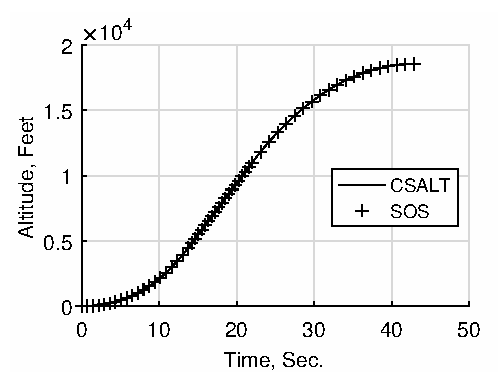
\includegraphics[width=\columnwidth]{../Figures/GoddardRocket_AlitudeVsTime}
    \caption{Altitude Comparison for Goddard Rocket Problem}
    \label{fig:goddard_alt}
\end{figure}
%
\begin{figure}
    \centering
    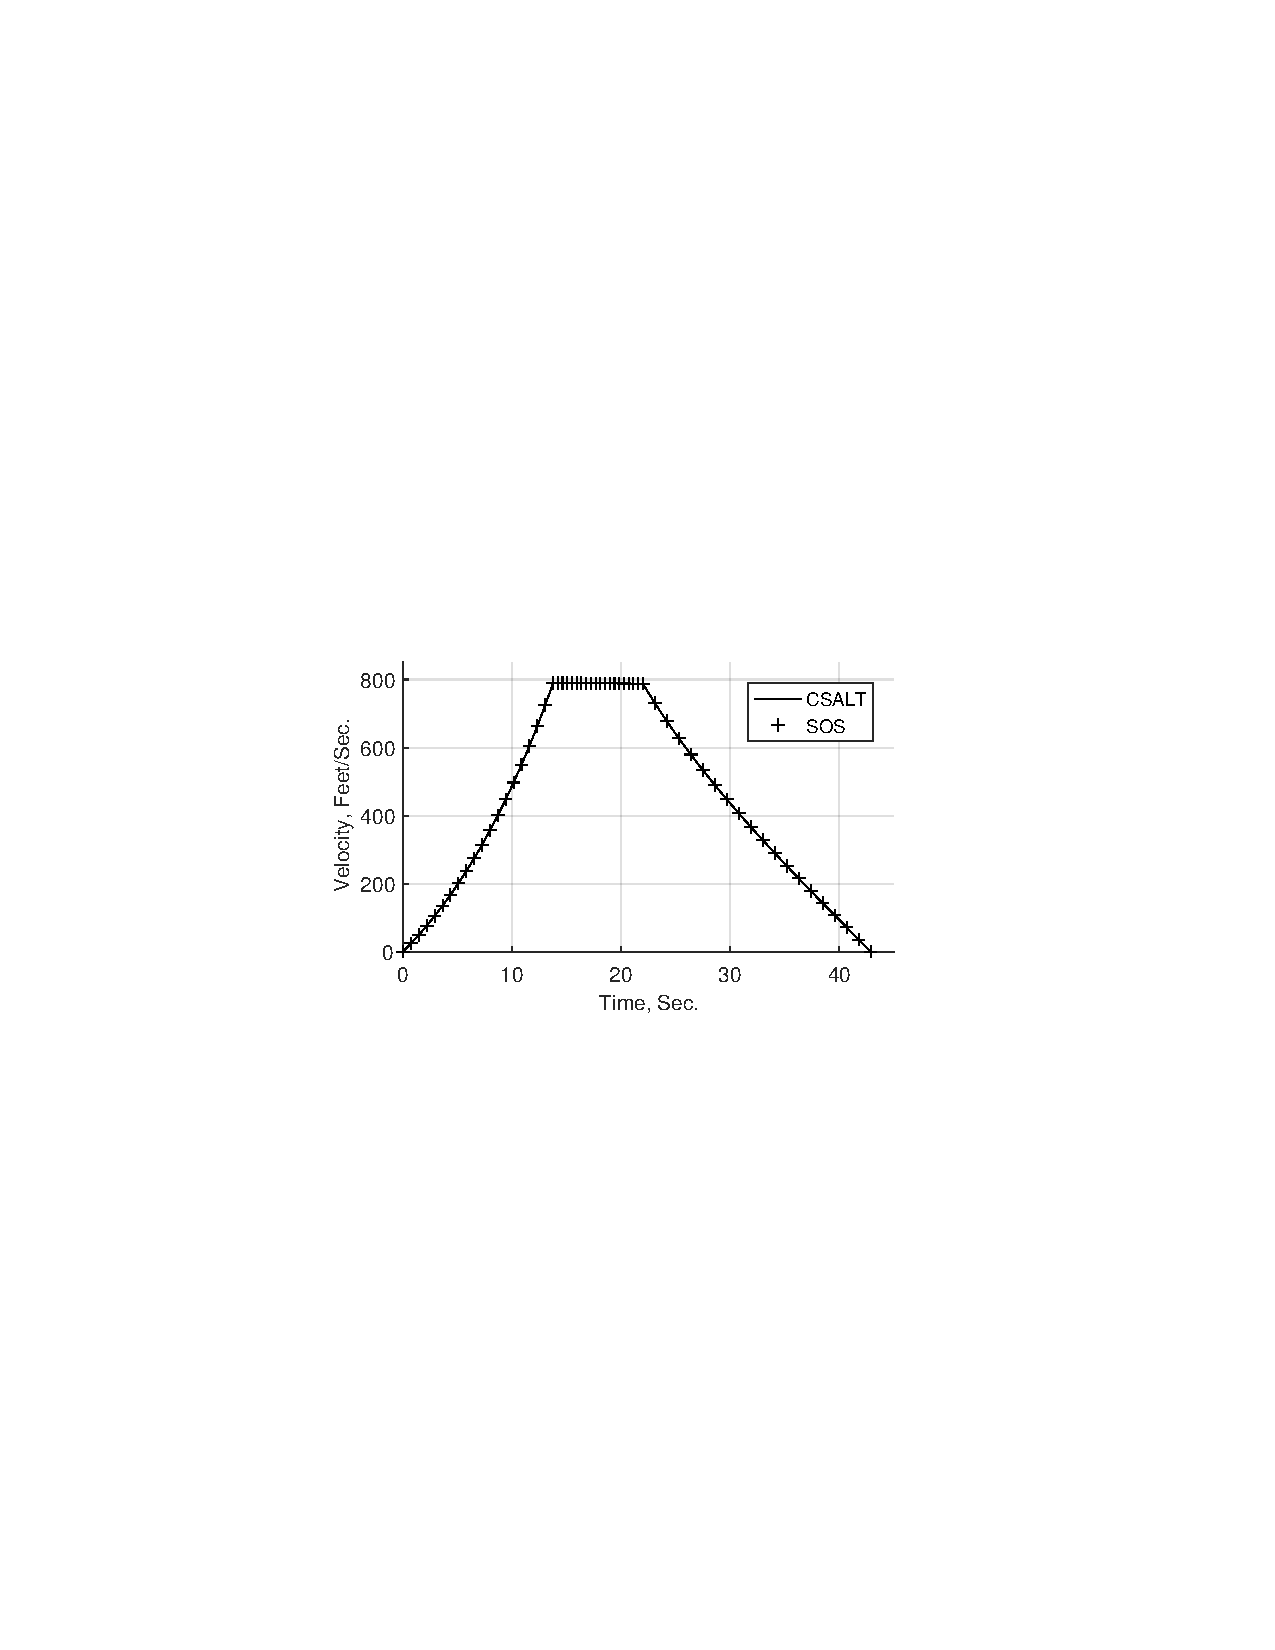
\includegraphics[width=\columnwidth]{../Figures/GoddardRocket_VelocityVsTime}
    \caption{Velocity Comparison for Goddard Rocket Problem}
    \label{fig:goddard_vel}
\end{figure}
%
\begin{figure}
    \centering
    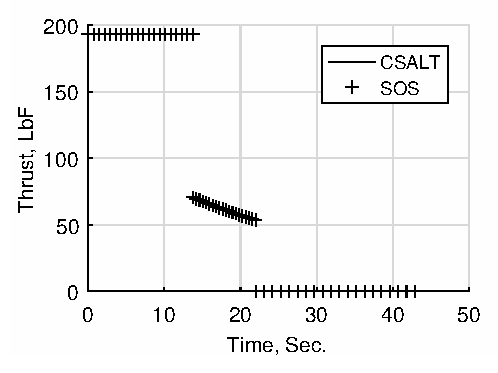
\includegraphics[width=\columnwidth]{../Figures/GoddardRocket_ThrustVsTime}
    \caption{Thrust Comparison for Goddard Rocket Problem}
    \label{fig:goddard_thrust}
\end{figure}

\subsection{Selected Low-Thrust Optimization Problems}

Low-thrust, solar electric propulsion (SEP) trajectories are among the most challenging optimal control problems. In general, exact solutions do not exist, but Horsewood and Dankanich\cite{Horsewood:a} have published results for certain industry standard problems. They used the indirect trajectory optimization software, HILTOP, which uses calculation of variations, to compare to a direct solver, MALTO \cite{Sims:a}, which uses an NLP solver to optimize multiple impulses to approximate a low-thrust trajectory. This section will discuss comparisons between these benchmark results and solutions found using CSALT.

The first problem considered is an Earth to Mars SEP transfer using two ion engines. The full problem specifications are not repeated here, and we refer the reader to Ref. \citeN{Horsewood:a} for a thorough description of the problem parameters. Note we did not replicate the low-thrust spiral to low Mars orbit because the benchmark studies did not perform optimization of that phase of the trajectory. The varying analytical models used modified the results sufficiently that it overshadowed the comparison of the optimal control history results themselves.
%
\begin{table}
	\centering
	\caption{Earth to Mars solutions comparison}
	\label{table:mars_comparison}
	\begin{tabularx}{\columnwidth}{lXXX}\bhline{.8pt}
		\textbf{Parameter} & \textbf{Malto} & \textbf{HILTOP} & \textbf{CSALT} \\\hline
		Launch date & 3/29/2022 & 4/7/2022 & 4/4/2022\\
		Launch C$_3$ (km$^2$/s$^2$) & 32.26 & 32.57 & 35.06\\
		Launch declination (deg) & -5.1 & -3.776 & -5.067\\
		Launch mass (kg) & 2,105.4 & 2,187.3 & 2,143.0\\
		Cruise flight time (days) & 458.2 & 455.7 & 452.0\\
		Cruise propellant (kg) & 324.3 & 338.7 & 336.9\\
		Mars Arrival date & 7/1/2023 & 7/6/2023 & 7/1/2023\\\bhline{.8pt}
	\end{tabularx}
\end{table}

The comparison of the Earth to Mars transfers using various optimal control software is presented in Table \ref{table:mars_comparison}. Qualitatively, CSALT converged to the same solution as the other tools. The launch dates, arrival dates, launch masses, and propellant masses all matched within a few days or tens of kilograms. The exact differences are within the expected margins of error of the modelling techniques. Malto uses discrete impulsive burn approximations, whereas the other two tools have smoothly varying control histories. This allows them to deliver more mass to Mars, as the NLP solver has greater flexibility. It is likely that with a greater number of time steps, Malto would have more closely approximated the solution of the other two tools. Both Malto and HILTOP are limited in their ability to scale their fidelity. For the purposes of comparison, the trajectory shown in CSALT used a similar level of modeling fidelity (2 body patched conic dynamics, polynomial thrust models), however, simple changes to the problem implementation would allow a higher fidelity solution.

The second trajectory benchmark problem considered is a re-optimization of the Dawn spacecraft\rq s trajectory. Recall that the Dawn spacecraft launched on September 27th of 2007, completed a Mars flyby and rendezvous with Vesta, before a final rendezvous with Ceres. Again, the full problem set-up is not repeated here, and can be found in Ref. \citeN{Horsewood:a}.
%
\begin{table}
    \centering
    \caption{Dawn mission solutions comparison}
    \label{table:dawn_comparison}
    \begin{tabularx}{\columnwidth}{lXXX}\bhline{.8pt}
        \textbf{Parameter} & \textbf{Malto} & \textbf{HILTOP} & \textbf{CSALT} \\\hline
        \textbf{Leg 1 Earth-Mars} & & & \\
        Launch date & 9/27/2007 & 9/27/2007 & 9/27/2007\\
        Launch C$_3$ (km$^2$/s$^2$) & 5.1529 & 5.2285 & 2.0862\\
        Launch declination (deg) & 28.5 & 28.5 & -11.1571\\
        Launch mass (kg) & 1,114.4 & 1,105.2 & 1227.2\\
        Flight time (days) & 510 & 510 & 527\\
        Arrival mass (kg) & 1,039.8 & 1,032.7 & 1132.5\\
        Propellant used (kg) & 74.6 & 72.4 & 94.7\\
        \textbf{Leg 2 Mars-Vesta} & & & \\
        Swingby date & 2/18/2009 & 2/18/2009 & 3/7/2009\\
        Swingby v$_\infty$ (km/s) & 4.10 & 4.11 & 4.49\\
        Passage altitude (km) & 300 & 300 & 300\\
        Flight time (days) & 894 & 827.7 & 846.4\\
        Arrival date & 8/1/2011 & 5/26/2011 & 7/11/2011\\
        Arrival mass (kg) & 907.3 & 901.4 & 986.1\\
        Propellant used (kg) & 132.5 & 131.3 & 146.4\\
        Stay time (days) & 270 & 336.3 & 270\\
        \textbf{Leg 3 Vesta-Ceres} & & & \\
        Departure date & 4/27/2012 & 4/27/2012 & 3/27/2012\\
        Flight time (days) & 1,038 & 1,038 & 1,067\\
        Arrival date & 2/28/2015 & 2/28/2015 & 2/28/2015\\
        Arrival mass (kg) & 807.2 & 802.3 & 879.6\\
        Propellant used (kg) & 100.1 & 99.1 & 106.5\\
        \textbf{Total Propellant (kg)} & \textbf{307.2} & \textbf{302.8} & \textbf{347.6}\\
        \textbf{Mission duration (days)} & \textbf{2,711} & \textbf{2,711} & \textbf{2,711}\\\bhline{.8pt}
    \end{tabularx}
\end{table}

Table \ref{table:dawn_comparison} compares the trajectories found in the same three optimal control solvers. In this case, CSALT found a qualitatively different trajectory. Whereas, both Malto and HILTOP determined that a higher energy (C3 $<$ 5 km$^2$/s$^2$) launch at the maximum allowable declination was optimal, CSALT proscribes a much lower energy launch to a relatively low declination. Due to the higher launch energy, the CSALT trajectory arrives at Mars using more propellant, and a cost of 17 days extra flight time. In the second leg of the journey, CSALT found a control history capable requiring roughly 16 kg more propellant in reaching a rendezvous with Vesta. The flight time was comparable to the Malto solution, but longer than the HILTOP solution. The final leg of the flight was somewhat different, as the CSALT trajectory required a greater amount of propellant to reach Ceres, in order to meet the arrival date constraint. However, the increased propellant on this final leg was not sufficient to compensate for savings elsewhere, and CSALT found a solution that would deliver almost 80 kg greater mass to Ceres, but requiring at least 40 kg more propellant.

\subsection{Selected IRK Problems}

In this section we present high level comparison results for the implicit Runge-Kutta (IRK) methods in CSALT.  The methods implemented are Trapezoid, Hermite-Simpson, and Runge-Kutta 4/6/8-th order algorithms all of type Lobatto IIIa. Table \ref{table:irk_comparison} presents the CSALT solutions for the Rao Automatica, Conway Orbit Example, and Interior Point problems obtained without mesh-refinement.  Mesh-refinement for IRK methods is underway but is not complete at the time of writing. The truth data for the problems illustrated here is contained in Table \ref{table:high_level_comparison2}.

In the absence of mesh-refinement, the quality of the solution is heavily affected by both the user-defined mesh points and the order of the collocation method. We expect that when employing the same mesh configuration, higher order methods will provide more accurate solutions than lower order methods and that is confirmed by the data in Table \ref{table:irk_comparison}.  CSALT solutions converge to the truth data as the order of the method increases when employing the same mesh. Note, the Hermite-Simpson method is a fourth order method similar to the Runge-Kutta 4th order method. Consequently, the results from Hermite-Simpson and the Runge-Kutta 4th order methods are effectively the same.
%
\begin{table}
    \centering
    \caption{IRK Solution Comparisons}
    \label{table:irk_comparison}
    \begin{tabularx}{\columnwidth}{Xccc}\bhline{.8pt}
    % \begin{tabularx}{\columnwidth}{Xp{.24\columnwidth}p{.24\columnwidth}p{.24\columnwidth}}\bhline{.8pt}
%        \multirow{2}{*}{\textbf{Method}} & \multirow{2}{.2\columnwidth}{\textbf{Rao Automatica}} & \multirow{2}{.2\columnwidth}{\textbf{Conway Orbit}} & \multirow{2}{.2\columnwidth}{\textbf{Interior Point}}\\\\\hline
                        & \textbf{Rao Automatica} & \textbf{Conway Orbit} & \textbf{Interior Point}\\\hline
        Trap.           & -6.3978783E-3           & 9.3879865E-2          & 9.2193588E-1\\
        HS              & -8.9985093E-3           & 9.5179464E-2          & 9.2053151E-1\\
        RK4             & -8.9985093E-3           & 9.5179464E-2          & 9.2053151E-1\\
        RK6             & -8.9636726E-3           & 9.5127025E-2          & 9.2053144E-1\\
        RK8             & -8.9637968E-3           & 9.5123433E-2          & 9.2053144E-1\\
        Truth           & -8.9637970E-3           & 9.5123383E-2          & 9.2053140E-1\\\bhline{.8pt}
    \end{tabularx}
\end{table}


Table \ref{table:irk_comparison2} contains test results for the trapezoidal method for Rao Automatica, Conway Orbit, and the Interior Point problems with the original mesh configuration, and a more dense mesh configuration expected to improve solution quality (effectively by-hand mesh refinement). The original solutions for Rao Automatica, Conway Orbit, and Interior Point use six, twenty, and ten, mesh points respectively. The improved solutions for Rao Automatica, Conway Orbit, and Interior Point use two hundred,
two hundred, and sixty, mesh points respectively.
%
\begin{table}
    \centering
    \caption{IRK Solution Comparisons Using Different Mesh Configurations}
    \label{table:irk_comparison2}
    \begin{tabularx}{\columnwidth}{Xccc}\bhline{.8pt}
    % \begin{tabularx}{\columnwidth}{Xp{.24\columnwidth}p{.24\columnwidth}p{.24\columnwidth}}\bhline{.8pt}
%        \multirow{2}{*}{\textbf{Method}} & \multirow{2}{.2\columnwidth}{\textbf{Rao Automatica}} & \multirow{2}{.2\columnwidth}{\textbf{Conway Orbit}} & \multirow{2}{.2\columnwidth}{\textbf{Interior Point}}\\\\\hline
        Solution        & \textbf{Rao } & \textbf{Conway } & \textbf{Interior Point}\\\hline
        Coarse          & -6.3978783E-3           & 9.3879865E-2          & 9.2193588E-1\\
        Fine            & -8.9621440E-3           & 9.5132015E-2          & 9.2056672E-1\\
        Truth           & -8.9637970E-3           & 9.5123383E-2          & 9.2053140E-1\\\bhline{.8pt}
    \end{tabularx}
\end{table}

\section{Future Work}

To date, CSALT development needs were prioritized based on the needs of low thrust interplanetary missions.  Future work will address other capabilities required for solving more general optimal control problems, including static and integral decision parameters and integral constraints.  We also plan to implement second derivatives and interfaces to NLP solvers that support full Newton methods.  Finally, in the spirit of not optimizing too early, we have not performed performance benchmarking or made performance-minded code changes.  We plan to address performance issues in the near future.

\section{Conclusions}

CSALT is mature software capable of solving a wide variety of optimization problems with high accuracy.  In this work, we compared CSALT solutions to a wide variety of problems, solved by a wide variety of approaches and tools.  In all cases, excellent agreement is seen, consistent with exact solutions or to the agreement between independent industry standards such as SOS and GPOPSII.  We demonstrated applications that employ both integral and algebraic cost functions, and algebraic point and path constraints.  Particular attention was given to low thrust orbit problems as CSALT is currently undergoing integration into the General Mission Analysis Tool for high-fidelity low thrust trajectory optimization.

\section*{Acknowledgments}\label{Acknowledgments}

The authors thank Dr. John Betts of Applied Mathematical Analysis, LLC for generous time spent in correspondence and for making available detailed solution data from the SOS package.  The authors also thank Dr. Anil Rao of the University of Florida for making available a free version of GPOPS II for benchmarking purposes and for time spent in correspondence regarding software implementation and testing. Contributions from KARI were supported by the National Research Foundation of Korea through the Lunar Exploration Development Program (NRF-2016M1A3A9926078).  Collaboration between NASA and KARI was performed under a Space Act Agreement.

\begin{thebibliography}{99}
\bibitem{Betts:a}
Betts, J.T.: Survey of Numerical Methods for Trajectory Optimization, Journal of Guidance, Control, and Dynamics, Vol. 21, March\text{-}April 1998, pp. 193\textendash207.
\bibitem{Hughes:a}
Hughes, S.P.,  Qureshi, R.H., Cooley, D.S., Parker, J.K., Grubb, T.G.: Verification and Validation of the General Mission Analysis Tool (GMAT),  AIAA/AAS Astrodynamics Specialist Conference, San Diego, CA, 2014.
\bibitem{Gill:a}
Gill, P. E., Murray, W., and Saunders, M. A.: SNOPT: An SQP algorithm for large-scale constrained optimization. SIAM Review 47, 1, 99\textendash131, 2002.
\bibitem{Betts:b}
Betts, J.T.: Practical Methods for Optimal Control and Estimation using Nonlinear Programming, 2nd Edition, Society for Industrial and Applied Mathematics, Philadelphia, 2010.
\bibitem{Betts:d}
Betts, J.T.: A Collection of Optimal Control Test Problems, http://appliedmathematicalanalysis.com/, 2015.
\bibitem{Betts:c}
Betts, J.T.: Sparse Optimization Suite (SOS) User Guide, http://appliedmathematicalanalysis.com/, 2016.
\bibitem{Betts:e}
Betts, J.T.: Using Direct Transcription to Compute Optimal Low Thrust Transfers Between Libration Point Orbits, Space Engineering: Modeling and Optimization with Case Studies, Springer International Publishing, 2016.
\bibitem{Becerra:a}
Becerra, V.M.: PSOPT Optimal Control User Manual, http://www.psopt.org, 2011.
\bibitem{Rao:a}
Patterson, M.A., Rao, A.V.: GPOPS-II: A MATLAB Software for Solving Multiple-Phase Optimal Control Problems Using hp-Adaptive Gaussian Quadrature Collocation Methods and Sparse Nonlinear Programming. ACM Trans. Math. Softw. 41, 1, Article 1, October 2014.
\bibitem{Rao:b}
Darby, C. L., Hager, W. W., Rao, A. V.: An hp-adaptive pseudospectral method for solving optimal control problems. Optimal Control Applications and Methods, 32, 4, 476\textendash502,2011.
\bibitem{Rao:c}
Patterson, M. A., Hager, W. W., and Rao, A. V.: A ph mesh refinement method for optimal control. Optimal Control Applications and Methods, 36, 4, 398\textendash421, 2015.
\bibitem{Horsewood:a}
Horsewood, J.L., Dankanich, J.W.: Heliocentric Interplanetary Low-thrust Optimization Program Capabilities and Comparison to NASA’s Low-thrust Trajectory Tools, 31st International Electric  Propulsion Conference, University of Michigan, Sept. 20\textendash24, 2009.
\bibitem{Nodecal:a}
Nocedal, J. , Wright, S. J.: Numerical Optimization, 2nd Edition. Springer. 2006.
\bibitem{Stryk:a}
Stryk, O.V., Bulirsch, R.: “Direct and indirect methods for trajectory optimization,” Annals of operations research, Vol. 37, No. 1, pp. 357\textendash373, 1992,
\bibitem{Garg:a}
Garg, D., Pattern, M. Hager, W.W., Rao, A.V, Benson, D.A, Huntington, G.T.: A unified framework for the numerical solution of optimal control problems using pseudospectral methods, Automatica,  46, pgs., 1843\textendash1851, 2010.
\bibitem{Hull:a}
Hull, D.G.: Optimal Control Theory for Applications, Springer, 2003.
\bibitem{Sims:a} Sims, J.A., Finlayson, P.A., Rinderle, E.A., Vavrina, M.A., Kowalkowski, T.D.: “Implementation of a low-thrust trajectory optimization algorithm for preliminary design,” AIAA/AAS Astrodynamics Specialist Conference and Exhibit, August 2006.
\end{thebibliography}

\end{document}
